En este capítulo se especifican las pruebas a las que se ha sometido el proyecto,
y las configuraciones y herramientas necesarias para poder llevarlas a cabo.

\section{Estrategia}

La estrategia de pruebas seguida es una serie de pruebas exhaustivas y
completas especificadas en un plan de pruebas, llevadas a cabo cada vez que se
modificaba algún componente importante y revisando todas las funcionalidades
repetidas veces en entornos asegurados.

\section{Entorno de pruebas}

Se distingue entre el entorno de pruebas de la API, que va a ser desplegada en
un único servidor, y el de la aplicación móvil, que puede ser desplegada en
multitud de dispositivos.

\subsection{API}

Para la utilización de entornos de prueba se ha optado por Vagrant, una
herramienta capaz de crear y configurar ambientes virtuales de manera sencilla,
reproducible y portátil. Permite desplegar el sistema necesario en una máquina
virtual tantas veces como se necesite y desde cualquier equipo que tenga Vagrant
instalado.

Esta herramienta tiene la ventaja de que permite crear las reglas de
configuración una única vez y reutilizarlas en casa ocasión, sin tener que volver
a desplegar el mismo sistema desde cero cada vez que se cambie de equipo.

El archivo principal de Vagrant es \texttt{Vagrantfile} que contiene la
configuración básica que se leerá cada vez que se ejecute un comando de Vagrant.

Vagrant permite utilizar multitud de plataformas de configuración, como Chef,
Puppet o Ansible. Hemos optado por esta última. Para poder utilizar Ansible para
definir las reglas de configuración del sistema hay que añadirlo a este archivo
de configuración:

\begin{minted}{bash}
  config.vm.provision "ansible" do |ansible|
    # ansible.sudo = true
    ansible.extra_vars = { ansible_ssh_user: 'vagrant',
    remote_user: 'vagrant', port_arg: PORT_NUMBER}
    ansible.raw_ssh_args = ["-o UserKnownHostsFile=/dev/null"]
    ansible.playbook = "provisioning/playbook.yml"
  end
\end{minted}

El archivo \texttt{playbook.yml} describe las reglas a seguir cada vez que se
despliegue un sistema. Este archivo puede contener tareas directamente o
llamadas a conjuntos de tareas, como es el caso.

\begin{minted}{bash}
---
- hosts: all
  vars_files:
    - vars.yml
  roles:
    - system
    - nginx
    - postgresql
    - django
    - gunicorn
    - supervisor
    - deploy
\end{minted}

Puede verse que se carga un archivo de variables y luego cada una de los
conjuntos de tareas. Se han organizado en función de los subsistemas que se
despliega con cada conjunto.

Una tarea puede tener los sigueintes atributos definidos en Yaml:
\begin{itemize}
\item \texttt{name}: nombre descriptivo de la tarea
\item \texttt{become}: ejecutar la tarea como otro usuario (si no se especifica,
  \texttt{become\_user}, se ejecutará como \texttt{root})
\item \texttt{command}: órden a ejecutar tal y como se escribiría en la terminal
\item \texttt{apt}: instalación de paquetes mediante \texttt{apt-get}
\item \texttt{git}: utilización de repositorios Git (clonado, pull, ...)
\item \texttt{stat}: utilización de archivos (creación, cambio de permisos,...)
\item \texttt{template}: utilización de plantillas (archivos con variables)
\end{itemize}

Por ejemplo, la configuración básica del sistema se encarga de:
\begin{enumerate}
\item Actualizar los paquetes del sistema.
\begin{minted}{bash}
- name: update and upgrading packages
  become: yes
  apt: update_cache=yes upgrade=safe
\end{minted}

\item Instalar los paquetes de python:
\begin{minted}{bash}
- name: install software-properties-common
  become: yes
  apt: pkg={{ item }} state=latest
  with_items: 
    - software-properties-common
    - python-setuptools
    - python-dev
- name: install pip3
  become: yes
  apt: pkg={{ item }} state=latest
  with_items:
    - python3-pip
    - python3-setuptools
- name: install pip again with easyintall
  become: yes
  command: python3 -m easy_install pip
\end{minted}

\item Instalar las dependencias de psycopg2:
\begin{minted}{bash}
- name: install dependencies for psycopg2
  become: yes
  apt: pkg=python-psycopg2 state=latest install_recommends=yes
\end{minted}
  
\item Instalar Git:
\begin{minted}{bash}
- name: install git
  become: yes
  apt: pkg=git state=latest
\end{minted}

\item Clonar el repositorio del proyecto:
\begin{minted}{bash}
- name: clone rep from GitHub
  git: accept_hostkey=true repo="{{ project_git_url }}"
       dest="~/{{ name_project }}"
\end{minted}

\item Asegurar la configuración supervisor:
\begin{minted}{bash}
- name: ensure supervisor is up to date
  become: yes
  apt: pkg=supervisor state=latest
- stat: path=/etc/supervisor/conf.d/{{ name_project }}.conf
  register: supervisor_conf
- name: ensure project stop
  when: supervisor_conf.stat.exists == True
  become: yes
  supervisorctl: name={{ name_project }} state=stopped
\end{minted}
  
\end{enumerate}

En el repositorio drf-vagrant-config puede verse la configuración completa.

Entonces, para ejecutar un entorno de pruebas aceptable, tan sólo hay que
ejecutar sobre la raíz del directorio \texttt{drf-vagrant-config}:

\begin{minted}{bash}
$ vagrant up
\end{minted}


\subsection{Aplicación móvil}

Para las pruebas sobre la aplicación móvil, dado que se realizan directamente
sobre el sistema en producción, el entorno coincide con los dispositivos de
prueba dispuestos en la sección~\ref{sec:costes} y diversos entornos variados de
otros probadores, según se especificará más adelante.


\section{Roles}

Se presentan dos roles principales necesarios para la ejecución de las pruebas.

\subsection{Probador principal}

La desarrolladora del proyecto es la principal probadora del sistema y de la
aplicación. Por un lado, es la encargado de desplegar y probar en el entorno
de pruebas de la API, teniendo la obligación de revisar las acciones y resolver
los conflictos que surjan. Además, ha de probar la aplicación móvil como si
fuera un usuario final más.

\subsection{Probadores externos}

Para más versatilidad, se ha utilizado el programa de betas de Google, a través
del cual se permite subir una aplicación móvil al Play Store, de forma que tan
sólo los usuarios a los cuales se les permita el acceso podrán descargar y
probar la aplicación.

\begin{figure}[htbp]
  \centering
  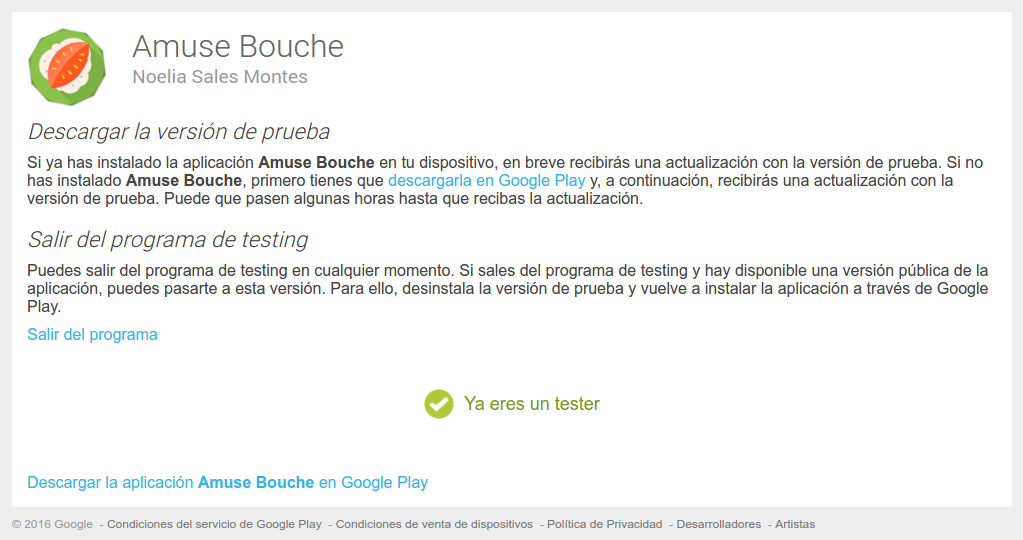
\includegraphics[width=\textwidth]{cap7/img/google-beta}
  \caption{Google Beta}
  \label{fig:google-beta}
\end{figure}

Los probadores externos han opinado sobre todos los aspectos de la aplicación,
incluyendo la interfaz de usuario, la usabilidad y la funcionalidad de esta.
Opiniones que siempre han sido tenidas en cuenta y han servido para mejorar
la aplicación.

Así, tenemos la seguridad de que la aplicación ha sido probada en dispositivos
muy variados.


\section{Pruebas funcionales}

\subsection{Pruebas de sistema}

Las pruebas de sistema, que buscan asegurar que el sistema cumple con todos
los requisitos establecidos, se desarrollaron de forma continua a medida que iba
avanzando el proyecto.

En cada iteración, las pruebas se ejecutaron sobre el entorno especificado y se
conectaron dispositivos para comprobar cómo se comportaba en condiciones
reales.

A continuación, se especifica el plan de pruebas completo con las validaciones
a comprobar por cada bloque funcional.

\begin{center}
  \begin{longtable}{|p{3.75cm}|p{3.5cm}|p{5.25cm}|p{1cm}|}
    \caption{Plan de pruebas del bloque funcional ``Usuarios''}\\
    \hline
    \textbf{Operación} & \textbf{Resultado} & \textbf{Validaciones} & \textbf{OK} \\
    \hline
    \endfirsthead
    \multicolumn{4}{c}{\tablename\ \thetable\ -- \textit{Continua desde la página anterior}} \\
    \hline
    \textbf{Operación} & \textbf{Resultado} & \textbf{Validaciones} & \textbf{OK} \\
    \hline
    \endhead
    \hline \multicolumn{4}{r}{\textit{Continua en la página siguiente}} \\
    \endfoot
    \hline
    \endlastfoot
    
    \textbf{Login}\newline
    El usuario introduce sus credenciales e inicia sesión en el sistema. &
    El usuario inicia sesión correctamente. &
    $\Box$ El usuario inicia sesión.\newline
    $\Box$ Se muestra la pantalla de bienvenida con el nombre y el correo
    electrónico del usuario y un botón de ``Cerrar sesión''.\newline
    $\Box$ El usuario aparece reflejado en el menú lateral donde antes ponía
    ``Login''. & \\

    & & $\Box$ Verificación de datos en tablas:
    \begin{itemize}
    \item AppData contiene una entrada con clave ``token'' y valor el
      token de autenticación devuelto por la API.
    \end{itemize} & \\ \hline
    
    \textbf{Login con errores}\newline
    El usuario introduce unas credenciales, pero no puede iniciar sesión. &
    Se muestra un mensaje de error. &
    $\Box$ Se muestra un mensaje de error indicando el problema.\newline
    El usuario no inicia sesión.\newline
    $\Box$ El usuario no aparece reflejado en el menú lateral, donde sigue
    apareciendo ``Login''. & \\ \hline

    \textbf{Registro}\newline
    El usuario introduce nuevos datos y se registra. &
    El usuario se registra correctamente. &
    $\Box$ El usuario se registra.\newline
    $\Box$ Se muestra la pantalla de login con un mensaje de que el registro ha
    sido exitoso.\newline
    $\Box$ Verificación de datos en API:
    \begin{itemize}
    \item Existe un nuevo usuario con los datos proporcionados por el usuario
    \end{itemize} & \\ \hline
    
    \textbf{Registro con errores}\newline
    El usuario introduce nuevos datos, pero no se puede registrar. &
    Se muestra un mensaje de error. &
    $\Box$ El usuario se registra.\newline
    $\Box$ Se muestra un mensaje de error indicando el problema. & \\ \hline
  \end{longtable}
\end{center}


\begin{center}
  \begin{longtable}{|p{3.75cm}|p{3.5cm}|p{5.25cm}|p{1.5cm}|}
    \caption{Plan de pruebas del bloque funcional ``Listado de recetas''}\\
    \hline
    \textbf{Operación} & \textbf{Resultado} & \textbf{Validaciones} & \textbf{OK} \\
    \hline
    \endfirsthead
    \multicolumn{4}{c}{\tablename\ \thetable\ -- \textit{Continua desde la página anterior}} \\
    \hline
    \textbf{Operación} & \textbf{Resultado} & \textbf{Validaciones} & \textbf{OK} \\
    \hline
    \endhead
    \hline \multicolumn{4}{r}{\textit{Continua en la página siguiente}} \\
    \endfoot
    \hline
    \endlastfoot
    
    \textbf{Recuperar listado de últimas recetas}\newline
    El usuario entra en la vista de ``Últimas recetas''. &
    Recupera el listado de recetas de la API. &
    $\Box$ Muestra el listado de recetas de la API.\newline
    $\Box$ Las recetas están ordenadas en función de las últimas
    actualizadas. & \\
    
    & & $\Box$ Se muestran las imágenes de las recetas o imágenes por defecto
    si no se pueden cargar bien. & \\ \hline

    \textbf{Recuperar listado de recetas descargadas}\newline
    El usuario entra en la vista de ``Descargadas''. &
    Recupera el listado de recetas de la base de datos. &
    $\Box$ Muestra el listado de recetas de la base de datos.\newline
    $\Box$ Las recetas están ordenadas en función de las últimas
    actualizadas.\newline
    $\Box$ Se muestran las imágenes de las recetas o imágenes por defecto si no
    se pueden cargar bien. & \\ \hline
    
    \textbf{Recuperar listado de mis recetas}\newline
    El usuario entra en la vista de ``Mis recetas''. &
    Recupera el listado de recetas de la base de datos que pertenecen al
    usuario. &
    $\Box$ Muestra el listado de recetas de la base de datos que pertenecen al
    usuario.\newline
    $\Box$ Las recetas están ordenadas en función de las últimas
    actualizadas.\newline
    $\Box$ Se muestran las imágenes de las recetas o imágenes por defecto si no
    se pueden cargar bien. & \\ \hline

    \textbf{Recuperar listado con errores}\newline
    El usuario entra en la vista de ``Últimas recetas'', ``Descargadas'' o ``Mis
    recetas'', pero no obtiene ninguna. &
    Se muestra un mensaje informando de que no hay recetas disponibles. &
    $\Box$ Se muestra un mensaje informando de que no hay recetas
    disponibles. & \\ \hline

    \textbf{Filtrar recetas}\newline
    El usuario selecciona criterios de filtrado en la vista lateral. &
    Recupera el listado de recetas de la API o de la base de datos que cumplan
    los criterios seleccionados. &
    $\Box$ Muestra el listado de recetas que cumplen los criterios. & \\ \hline
  \end{longtable}
\end{center}


\begin{center}
  \begin{longtable}{|p{3.75cm}|p{3.5cm}|p{5.25cm}|p{1.5cm}|}
    \caption{Plan de pruebas del bloque funcional ``Detalle de una receta''}\\
    \hline
    \textbf{Operación} & \textbf{Resultado} & \textbf{Validaciones} & \textbf{OK} \\
    \hline
    \endfirsthead
    \multicolumn{4}{c}{\tablename\ \thetable\ -- \textit{Continua desde la página anterior}} \\
    \hline
    \textbf{Operación} & \textbf{Resultado} & \textbf{Validaciones} & \textbf{OK} \\
    \hline
    \endhead
    \hline \multicolumn{4}{r}{\textit{Continua en la página siguiente}} \\
    \endfoot
    \hline
    \endlastfoot
    
    \textbf{Ver detalle de una receta}\newline
    El usuario selecciona una receta del listado. &
    Se accede a la vista de detalle con los datos de la receta. &
    $\Box$ Se muestra el detalle de la receta.\newline
    $\Box$ Se muestran los comentarios de la receta si tiene definido el
    identificador de la API.\newline
    $\Box$ Se muestra el icono de ``Editar receta'' si la receta no existe en
    la base de datos o si existe en la base de datos pero está más actualizada
    en la API.\newline
    $\Box$ Se muestra el icono de ``Descargar receta'' si la receta no existe en
    la base de datos o si existe pero está más actualizada en la API.\newline
    $\Box$ Se muestra el icono de ``Subir receta'' si la receta no existe en la
    API o si existe pero está más actualizada en la base de datos.\newline
    $\Box$ Se muestra el icono de ``Puntuar receta'' si el usuario ha iniciado
    sesión.\newline
    $\Box$ Se muestra el icono de ``Editar receta'' si la receta se encuentra en
    la base de datos y el usuario de la receta es el usuario actual.\newline
    $\Box$ Se muestra el icono de ``Borrar receta'' si la receta se encuentra en
    la base de datos.
    & \\ \hline
    
    \textbf{Editar receta}\newline
    El usuario selecciona el icono de ``Editar receta''. &
    Se accede a la vista de edición con los datos de la receta. &
    $\Box$ Se muestra la vista de edición de la receta.
    & \\ \hline

    \textbf{Descargar receta}\newline
    El usuario selecciona el icono de ``Descargar receta''. &
    Se descargan los datos de la receta. &
    $\Box$ Se descargan los datos de la receta.\newline
    $\Box$ Se actualiza la vista de detalle para mostrar los datos
    actualizados.\newline
    $\Box$ Verificación de datos en la base de datos:
    \begin{itemize}
    \item Recipe: Se actualiza la receta con los nuevos datos.
    \item RecipeCategory: Se actualizan las categorías de la receta.
    \item RecipeIngredient: Se actualizan los ingredientes de la receta.
    \item RecipeDirection: Se actualizan los pasos de la receta.
    \end{itemize}
    & \\ \hline

    \textbf{Descargar receta con errores}\newline
    El usuario selecciona el icono de ``Descargar receta'', pero no se descarga
    nada.&
    Se muestra un error informando de lo ocurrido. &
    $\Box$ Se muestra un error informando de que no se ha descargado la
    receta. & \\ \hline

    \textbf{Subir receta}\newline
    El usuario selecciona el icono de ``Subir receta''. &
    Se suben los datos de la receta a la API. &
    $\Box$ Se envían los datos de la receta.\newline
    $\Box$ Se informa de que se han enviado correctamente.\newline
    $\Box$ Verificación de datos en la API:
    \begin{itemize}
    \item Recipe: Se actualiza la receta con los nuevos datos o se crea si no
      existía.
    \item RecipeCategory: Se actualizan las categorías de la receta o se crean
      si no existía la receta.
    \item RecipeIngredient: Se actualizan los ingredientes de la receta o se
      crean si no existía la receta.
    \item RecipeDirection: Se actualizan los pasos de la receta o se crean
      si no existía la receta.
    \end{itemize}
    & \\ \hline

    \textbf{Subir receta con errores}\newline
    El usuario selecciona el icono de ``Subir receta'', pero no se registra
    correctamente &
    Se muestra un error informando de lo ocurrido. &
    $\Box$ Se muestra un error informando de que no se ha registrado la
    receta. & \\ \hline

    \textbf{Puntuar receta}\newline
    El usuario selecciona el icono de ``Puntuar receta'', selecciona la
    valoración y acepta. &
    Se envía una nueva valoración. &
    $\Box$ Se envían los datos de la valoración de la receta.\newline
    $\Box$ Se informa de que se han enviado correctamente.\newline
    $\Box$ Se muestra la actualización de la valoración en la vista de
    detalle.\newline
    $\Box$ Verificación de datos en la API:
    \begin{itemize}
    \item RecipeRating: Se añade una nueva valoración.
    \item Recipe: Se actualizan los datos de las valoraciones generales.
    \end{itemize}
    & \\ \hline
    
    \textbf{Puntuar receta con errores}\newline
    El usuario selecciona el icono de ``Puntuar receta'', selecciona la
    valoración y acepta, pero no funciona correctamente. &
    Se muestra un error informando de lo ocurrido. &
    $\Box$ Se muestra un error informando de que no se ha registrado la nueva
    puntuación.& \\ \hline

    \textbf{Borrar receta}\newline
    El usuario selecciona el icono de ``Borrar receta''. Aparece un mensaje de
    confirmación y acepta. &
    Se borra la receta. &
    $\Box$ Se borra la receta de la base de datos.\newline
    $\Box$ Se vuelve a la vista de listado anterior. \newline
    $\Box$ Verificación de datos en la base de datos:
    \begin{itemize}
    \item Recipe: Se elimina el registro de la receta actual.
    \end{itemize}
    & \\ \hline
    
    \textbf{Enviar comentario}\newline
    El usuario introduce un comentario en el campo de texto y selecciona el
    botón de ``Enviar comentario''. &
    Se envía un nuevo comentario. &
    $\Box$ Se envían los datos del comentario de la receta.\newline
    $\Box$ Se informa de que se han enviado correctamente.\newline
    $\Box$ Se muestra la actualización de la valoración en la vista de
    detalle de los comentarios.\newline
    $\Box$ Verificación de datos en la API:
    \begin{itemize}
    \item RecipeComment: Se añade un nuevo comentario.
    \end{itemize}
    & \\ \hline

    \textbf{Enviar comentario con errores}\newline
    El usuario introduce un comentario en el campo de texto y selecciona el
    botón de ``Enviar comentario'', pero no funciona correctamente. &
    Se muestra un error informando de lo ocurrido. &
    $\Box$ Se muestra un error informando de que no se ha registrado el nuevo
    comentario. & \\ \hline

    \textbf{Mostrar imagen de un paso}\newline
    El usuario selecciona el icono de ``Imagen'' de un paso de la receta. &
    Se muestra la imagen que corresponda. &
    $\Box$ Se muestra la imagen definida en el paso de la receta.
    & \\ \hline
    
    \textbf{Mostrar video de un paso}\newline
    El usuario selecciona el icono de ``Video'' de un paso de la receta. &
    Se muestra el video que corresponda. &
    $\Box$ Se muestra el video definida en el paso de la receta.
    & \\ \hline

    \textbf{Activar cronómetro de un paso}\newline
    El usuario selecciona el icono de ``Cronómetro'' de un paso de la receta. &
    Se muestra el cronómetro y se activa. &
    $\Box$ Se muestra el cronómetro con el tiempo indicado en el paso de la
    receta.\newline
    $\Box$ Se muestra un botón de ``Saltar'' para evitar seguir esperando a que
    termine el cronómetro.    
    & \\ \hline

    \textbf{Activar lectura de un paso}\newline
    El usuario selecciona el icono de ``Lectura'' de un paso de la receta. &
    Se lee la descripción del paso. &
    $\Box$ Se lee la descripción indicada en el paso de la receta.
    & \\ \hline
    
    \textbf{Activar lectura continua}\newline
    El usuario selecciona el icono de ``Lectura continua''. &
    Se activa el modo de lectura continua. &
    $\Box$ Se lee la descripción del primer paso de la receta.\newline
    $\Box$ Se activa el cronómetro si el paso tiene tiempo definido.\newline
    $\Box$ Se muestra el diálogo de captura de órdenes y se espera a que el
    usuario seleccione una por voz o por pantalla.\newline
    $\Box$ Se ejecuta la siguiente orden.\newline
    $\Box$ Se sigue el bucle hasta que se llegue al último paso o hasta que el
    usuario selecciona la orden ``Salir''.\newline
    & \\ \hline
    
  \end{longtable}
\end{center}


\begin{center}
  \begin{longtable}{|p{3.75cm}|p{3.5cm}|p{5.25cm}|p{1.5cm}|}
    \caption{Plan de pruebas del bloque funcional: ``Edición de una receta''}\\
    \hline
    \textbf{Operación} & \textbf{Resultado} & \textbf{Validaciones} & \textbf{OK} \\
    \hline
    \endfirsthead
    \multicolumn{4}{c}{\tablename\ \thetable\ -- \textit{Continua desde la página anterior}} \\
    \hline
    \textbf{Operación} & \textbf{Resultado} & \textbf{Validaciones} & \textbf{OK} \\
    \hline
    \endhead
    \hline \multicolumn{4}{r}{\textit{Continua en la página siguiente}} \\
    \endfoot
    \hline
    \endlastfoot
    
    \textbf{Editar atributo}\newline
    El usuario añade un nuevo valor a un atributo de la receta. &
    El usuario añade un nuevo valor a un atributo de la receta. &
    $\Box$ Se valida el valor del atributo de la receta.\newline
    $\Box$ Se muestra el estado de la validación junto al atributo (válido
    o no válido).
    & \\ \hline

    \textbf{Añadir ingrediente}\newline
    El usuario selecciona ``Añadir ingrediente''. Aparece el diálogo de añadir
    ingrediente, introduce los datos necesario y acepta. &
    El usuario añade un nuevo ingrediente a la receta. &
    $\Box$ Se añade un nuevo ingrediente a la receta.\newline
    $\Box$ Se busca en la base de datos el nuevo ingrediente para obtener sus
    categorías relacionadas y se añaden a la receta.\newline
    $\Box$ Se actualiza la vista para mostrar el nuevo ingrediente y las nuevas
    categorías.
    & \\ \hline

    \textbf{Borrar ingrediente}\newline
    El usuario selecciona el icono de ``Borrar'' de un ingrediente. &
    Se borra un ingrediente a la receta. &
    $\Box$ Se busca en la base de datos todos los ingredientes de la receta para
    verificar si todas las categorías que tiene deben seguir.\newline
    $\Box$ Se actualiza la vista para mostrar la desaparición del ingrediente y
    de las categorías afectadas.
    & \\ \hline
    
    \textbf{Añadir paso}\newline
    El usuario selecciona ``Añadir paso. Aparece el diálogo de añadir
    paso, introduce los datos necesario y acepta. &
    El usuario añade un nuevo paso a la receta. &
    $\Box$ Se añade un nuevo paso a la receta.\newline
    $\Box$ Se actualiza la vista para mostrar el nuevo paso.
    & \\ \hline

    \textbf{Borrar paso}\newline
    El usuario selecciona el icono de ``Borrar'' de un paso. &
    Se borra un paso a la receta. &
    $\Box$ Se actualiza la vista para mostrar la desaparición del paso.
    & \\ \hline
    
    \textbf{Guardar receta}\newline
    El usuario selecciona el icono de ``Guardar receta''. &
    Se guarda la receta. &
    $\Box$ Se actualizan los datos de la receta en la base de datos (o se
    crea si no existía).\newline
    $\Box$ Se muestra un mensaje indicando que se ha guardado
    correctamente.\newline
    $\Box$ Verificación de datos en la base de datos:
    \begin{itemize}
    \item Recipe: Se actualiza o añade la receta con los datos indicados.
    \item RecipeCategory: Se actualizan las categorías de la receta o se crean
      si no existía la receta.
    \item RecipeIngredient: Se actualizan los ingredientes de la receta o se
      crean si no existía la receta.
    \end{itemize}
    & \\ \hline
    
    & & 
    \begin{itemize}
    \item RecipeDirection: Se actualizan los pasos de la receta o se crean
      si no existía la receta.
    \end{itemize}    
    & \\ \hline
  \end{longtable}
\end{center}

    
\subsection{Pruebas de aceptación}

Para verificar que el producto estaba listo para el paso a producción, se hizo
un despliegue en un servidor real y se abrió la beta de Google para confirmar
que el sistema funciona con varios usuarios usando la aplicación móvil
simultáneamente. El servidor ha permanecido online desde principios del mes de
julio hasta la fecha.


\section{Pruebas no funcionales}

Las pruebas no funcionales buscan verificar aspectos del proyecto más allá de su
funcionalidad, como la seguridad o la calidad del código.

\subsection{Pruebas de seguridad}

Las pruebas de seguridad sirven para verificar que la información de los
usuarios y las áreas privadas de la API son seguras. Entre las pruebas que se
realizaron se encuentran las siguientes:
\begin{itemize}
\item Se intentó acceder a URLs de la zona de usuarios autenticados sin tener
  un token válido. Por ejemplo, al intentar acceder a la URL
  \url{http://amuse-bouche.noeliarcado.es/auth/me/} da un error 403 con la
  siguiente respuesta:
  \begin{minted}{bash}
{"detail":"Authentication credentials were not provided."}
  \end{minted}

\item Se intentó iniciar sesión con credenciales inválidas. La petición devuelve
  un error 403 con el siguiente mensaje:
  \begin{minted}{bash}
$ curl -X POST http://amuse-bouche.noeliarcado.es/auth/login/
    --data 'username=test&password=wrong_password'

{"non_field_errors":["Unable to login with provided credentials."]}
  \end{minted}

\item Se intentó iniciar sesión con credenciales válidas. La petición devuelve un
  200 con el token de autenticación:

  \begin{minted}{bash}
$ curl -X POST http://amuse-bouche.noeliarcado.es/auth/login/ \
    --data 'username=test&password=password'

    {"auth_token":"token"}

    
$ curl -X GET http://amuse-bouche.noeliarcado.es/auth/me/ \
    -H 'Authorization: Token token'
    
{"email":"test@gmail.com","first_name":"test","last_name":"test",
 "id":3,"username":"test"}%  
  \end{minted}

\item Se intentó acceder al \textit{endpoint} de recetas utilizando varios
  métodos con el siguiente resultado:

  \begin{itemize}
  \item Método GET: Devuelve el listado de recetas correctamente, enviando un
    \textit{token} de autenticación o no.

  \item Métodos POST, PUT y DELETE: Devuelve error 403 con credenciales inválidas o sin
    credenciales.

    \begin{minted}{bash}
$ curl -X METHOD http://amuse-bouche.noeliarcado.es/recipes/1/ \
      -H 'Authorization: Token token'

{"detail":"Authentication credentials were not provided."}            
    \end{minted}

    Si las credenciales son válidas, pero el usuario no es el poseedor de la
    receta, devuelve un error 403 con el sigiente mensaje:

    \begin{minted}{bash}
$ curl -X METHOD http://amuse-bouche.noeliarcado.es/recipes/1/ \
      -H 'Authorization: Token token'

{"detail":"You do not have permission to perform this action."}%               
    \end{minted}

    Si las credenciales son válidas y el usuario es el poseedor de la receta,
    se devuelve un código 200 y se efectúa la operación correctamente..

    \begin{minted}{bash}
$ curl -X METHOD http://amuse-bouche.noeliarcado.es/recipes/1/ \
      -H 'Authorization: Token token'    
    \end{minted}
    
  \end{itemize}

\item Se intentó acceder a los \textit{endpoints} de comentarios y puntuaciones
  con el siguiente resultado:

  \begin{itemize}
  \item Método GET: Devuelve el listado de comentarios (o puntuaciones)
    correctamente, enviando un \textit{token} de autenticación o no.

  \item Métodos POST y PUT: Devuelve error 403 con credenciales
    inválidas o sin credenciales.

    \begin{minted}{bash}
$ curl -X METHOD http://amuse-bouche.noeliarcado.es/recipes/1/ \
      -H 'Authorization: Token token'

{"detail":"Authentication credentials were not provided."}            
    \end{minted}

    Si las credenciales son válidas, se devuelve un código 200 y se efectúa la
    operación correctamente..

    \begin{minted}{bash}
$ curl -X METHOD http://amuse-bouche.noeliarcado.es/recipes/1/ \
      -H 'Authorization: Token token'    
    \end{minted}

  \item Método DELETE: Devuelve error 403 con credenciales inválidas o sin
    credenciales.

    \begin{minted}{bash}
$ curl -X METHOD http://amuse-bouche.noeliarcado.es/translations/1/ \
      -H 'Authorization: Token token'

{"detail":"Authentication credentials were not provided."}            
    \end{minted}

    Si las credenciales son válidas y el usuario forma parte del grupo de
    Moderadores, se devuelve un código 200 y se efectúa la operación correctamente.

    \begin{minted}{bash}
$ curl -X METHOD http://amuse-bouche.noeliarcado.es/recipes/1/ \
      -H 'Authorization: Token token'    
    \end{minted}
  \end{itemize}

  
\item Se intentó acceder al \textit{endpoint} de traducciones
  con el siguiente resultado:
  
  \begin{itemize}
  \item Método GET: Devuelve el listado de traducciones correctamente, enviando
    un \textit{token} de autenticación o no.

  \item Métodos POST, PUT y DELETE: Devuelve error 403 con credenciales inválidas o sin
    credenciales.

    \begin{minted}{bash}
$ curl -X METHOD http://amuse-bouche.noeliarcado.es/translations/1/ \
      -H 'Authorization: Token token'

{"detail":"Authentication credentials were not provided."}            
    \end{minted}

    Si las credenciales son válidas, pero el usuario no es el poseedor de la
    receta, devuelve un error 403 con el sigiente mensaje:

    \begin{minted}{bash}
$ curl -X METHOD http://amuse-bouche.noeliarcado.es/recipes/18/ \
      -H 'Authorization: Token token'

{"detail":"You do not have permission to perform this action."}%               
    \end{minted}

    Si las credenciales son válidas y el usuario forma parte del grupo de
    Moderadores, se devuelve un código 200 y se efectúa la operación correctamente.

    \begin{minted}{bash}
$ curl -X METHOD http://amuse-bouche.noeliarcado.es/recipes/1/ \
      -H 'Authorization: Token token'    
    \end{minted}
    
  \end{itemize}
  
\item Se intentó acceder al \textit{endpoint} de ingredientes e independientemente
  del método utilizado, siempre devuelve error 403 a menos que el usuario
  cuyo \textit{token} se envíe sea del grupo de moderadores.
\item Se intentó acceder al \textit{endpoint} de usuarios e independientemente
  del método utilizado, siempre devuelve error 403 a menos que el usuario
  cuyo \textit{token} se envíe sea del grupo de moderadores.
\end{itemize}

\subsection{Verificación de la calidad del código}

Para el código Python, utilizando \textbf{pylint} y \textbf{python-mode} en
Emacs se revisa cada fichero de código conforme se va desarrollando para
comprobar que no existan fallos y además para satisfacer el estándar PEP8 de
codificación. Se comprueban características como puede ser la longitud del
código de línea, la comprobación de que los nombres de variables sean
gramaticalmente correctos según su estándar de codificación, o la comprobación
de que las interfaces declaradas sean realmente puestas en práctica, entre otras
cosas.

Para el código Java, se emplea el propio Android Studio que trae sus propios
verificadores y resaltadores de serie.
